\chapter{Introduction} % Main chapter title
\label{Chapter1}
\lhead{Chapter 1. \emph{Introduction}} % Change X to a consecutive number; this is for the header on each page - perhaps a shortened title

\section{Background}
Computer simulations~\cite{compsim} have been an inseparable part of scientific research since the advent of computing machines. They serve as a valuable tool and a helping hand in understanding physical phenomena, ranging from the development of modern vaccines~\cite{hollingsworth2018molecular} to the design of advanced aerospace systems and the prediction of complex climate patterns. The basis of this technique is to define a mathematical model and to perform a series of step-by-step procedures to obtain a numerical solution. By leveraging sophisticated algorithms and high-performance computing resources, simulations facilitate the investigation of intricate systems with remarkable precision and efficiency. Simulation results have become indispensable for informed decision-making, policy formulation, and technological innovation in many disciplines.

\section{Atomistic Simulations}
Simulations at an atomistic level are designed to understand the principles of the science of atoms and molecules, by which they interact with each other in various chemical phenomena. These provide a framework for understanding the connection between forces, energies, and potential fields with the observed properties. For example, \ac{MD}~\cite{MDsim} simulations are an important technique that determines the motion of many-body macroscopic systems obeying classical mechanics.  Through this approach, the trajectories of atoms and molecules are computed over time, enabling the study of structural, thermodynamic, and kinetic properties of matter. Molecular simulations provide a dynamic picture of systems that complements static experimental observations by accurately modelling interatomic forces and integrating the equations of motion. It is a valuable tool offering insights into molecular behaviour at the atomic scale, and can be used to design systems in tandem with experiments. 

To achieve meaningful and accurate molecular simulations, defining appropriate models and equations that describe the subject system is essential. These modelling equations typically incorporate long-range interactions, such as van der Waals forces and Coulombic interactions, which will be discussed in the subsequent section.

% \swb{What you have written is fine. I will encourage you to add lots of citations.}
% @@@I agree, this section needs a lot of citations. I have rewritten a few portions.@@@

\section{Long Range Interactions}
The term long-range interactions in chemical physics refers to electrostatic potential energies between ions that vary with the inverse power of the distance ($r$) between them, or as $r^{-d}$, where \textit{d} is the dimensionality of the system \cite{simulation_of_liq}. Because these interactions are common in physical systems, it is essential to model them correctly. However, they also represent one of the most serious difficulties in \ac{MD} simulations. In bulk systems, each ion effectively interacts with an infinite number of neighbours. Trying to compute these interactions directly leads to a sum over infinitely many contributions. This is not only computationally unmanageable but also mathematically problematic, since the total Coulomb energy in three dimensions is conditionally convergent, meaning its value depends on the order in which the contributions are added. As a result, naïvely truncating the interactions at some large distance can produce misleading or incorrect results.
% \subsection{\ac{PBC}}
\subsection{Periodic Boundary Conditions}
To tackle the fundamental challenge of simulating an infinite system with a manageable number of particles, simulations typically employ \ac{PBC}. Under this approximation, the simulation box is repeated throughout the space to mimic a bulk or infinite system, forming an infinite periodic structure. The motion of the atoms in the original box is replicated in all of its other periodic images. Particles that leave one side of the box re-enter from the opposite side. This approach eliminates edge effects without requiring explicit surface molecules.
\begin{figure}
    \centering
    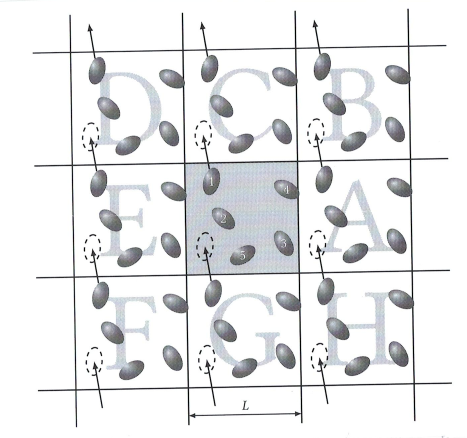
\includegraphics[width=0.75\linewidth]{images/periodic.png}
    \caption{A two-dimensional system with periodic boundaries, where molecules are free to move in and out through any of the four sides of each box. The figure is
 adapted from ``Computer Simulation of Liquids''~\cite{simulation_of_liq}.}
    \label{fig:periodic}
\end{figure}
\subsection{Minimum Image Convention}
The \ac{MIC}~\cite{minimumimage,hloucha1998fast} is a simple but powerful rule used under periodic boundary conditions. It states that each particle should only interact with the nearest periodic image of every other particle. In practice, for every pair of particles, we compute the distance considering the closest image among all the periodic copies. This avoids double-counting and ensures that no interaction is calculated more than once. MIC is especially efficient for short-range potentials, where interactions beyond a certain cut-off are negligible. 

\subsection{Significance}
Proper treatment of long-range interactions is essential, as they govern key structural and thermodynamic properties of liquids, ionic systems, and biomolecules. Periodic boundary conditions allow a finite system to mimic bulk behaviour by eliminating surface effects, while the minimum image convention ensures interactions are computed efficiently and without ambiguity. Together, these methods enable accurate and physically meaningful simulations of infinite systems using a tractable number of particles.

\section{Motivation of the Thesis}
Understanding electrostatic interactions in restricted and interfacial systems is fundamental to numerous areas in physical chemistry, materials science, and biophysics. A key example is \ac{EDL}~\cite{EDLbook,stillinger1960theory,grahame1947electrical}: a morphological arrangement of charged atoms that forms at the interface between a charged surface and an adjacent electrolytic solution. This phenomenon governs foundational laws in colloid science, electrochemistry, and interfacial physics. 

The generally accepted model of EDL comprises of the Stern layer~\cite{stern1924theorie,helmholtz1853ueber} (or compact layer), where specifically adsorbed ions (and sometimes solvent molecules) are located immediately next to the charged surface, and the diffuse layer (or Gouy-Chapman layer), which extends into the bulk liquid with ion distributions governed by a balance of electrostatic forces and thermal motion. The simulations of EDL, however, would require a restricted periodicity in two dimensions. Accurately simulating large-scale physical systems with restricted periodicity remains a central challenge in computational science, despite the rapid evolution of computer hardware. While hardware improvements have enhanced computational capabilities, they are not sufficient on their own to overcome the scaling limitations inherent in modelling complex interactions. Since the computational effort required to compute long-range coulombic interactions scales quadratically with the number of ions, developing algorithms that significantly reduce these costs, particularly for systems that exhibit reduced periodicities, is essential. 

\section{Objective of the Thesis}
The conventional approach for modelling slab geometries introduces a dipole correction \cite{dipole-yeh-berkowitz} to the Coulomb interactions within a fully periodic framework with vacuum padding in the non-periodic direction. Alternatively, exact formulations of the Ewald summation~\cite{Ewald1921} have been developed for systems with two-dimensional periodicity \cite{kawata, PARRY1975433,de1979electrostatic, Heyes19771485}, rigorously accounting for the anisotropic boundary conditions inherent to slab configurations. These methods accurately capture long-range electrostatics without relying on artificial corrections; however, their computational cost typically exceeds $O(NlogN)$~\cite{huang2024pmc}, rendering them impractical for large-scale simulations.

The primary objective of this thesis is to develop and implement an exact 2D Ewald summation algorithm that achieves the \emph{same} computational complexity as the traditional 3D Ewald method, while offering improved efficiency and scalability. Additionally, this work focuses on writing high-performance, optimized code, emphasizing efficient memory access, vectorization, and cache-friendly data structures, and further optimizing the computational performance through parallelization using OpenMP~\cite{dagum1998openmp}. Through the development of novel algorithm tailored for 2D periodic systems, combined with low-level code optimizations facilitated by performance profiling using Intel\textsuperscript{\textregistered} VTune~\cite{VTUNE} and parallelization using OpenMP, this thesis aims to provide a robust and practical framework for large-scale \acs{MD} simulations that can be useful to study some fundamental physical and chemical phenomena like thin films, surface science,  electrochemical interfaces and adsorption.

\section{Organization of the Thesis}
This thesis is organized into six chapters as outlined below:

\autoref{Chapter1} develops the background and context for this study, discussing Molecular Simulation and its application, and the significance of long-range interactions such as Coulombic forces. It introduces the key concepts like \ac{PBC} and \ac{MIC}. This chapter also highlights the motivation and objectives of this thesis.

\autoref{Chapter2} reviews the theoretical foundations and computational strategies for treating Coulombic interactions in molecular simulations. It provides a detailed discussion of the Ewald summation method, including its formulations for fully periodic and slab-type systems. Additionally, it describes the particle mesh algorithms (\acs{SPME} and \acs{2D-PME}) designed to efficiently compute long-range electrostatics in these respective geometries.

\autoref{Chapter3}: presents the novel approach to Ewald summation for slab systems. It covers the mathematical framework and optimal parameter selection, and provides insights into the specific aspects of the method that improve its computational efficiency. 

\autoref{Chapter4} presents numerical experiments to assess the accuracy and computational efficiency of the developed method. It examines convergence behaviour, improvements in the real-space calculations, modifications to the Particle Mesh Ewald approach, and scaling with respect to system size.

\autoref{Chapter5} focuses on the program implementation and optimization of the proposed method. It begins with an analysis of performance hotspots in the baseline program and then describes the various optimization techniques applied, including vectorization and parallelization using OpenMP. The chapter concludes with a performance evaluation that highlights the effectiveness of these optimizations and the improvements achieved through parallelization.

\autoref{Chapter6} summarizes the key findings and contributions of this work.